\documentclass[aspectratio=169,10pt]{beamer}
\usepackage{fontspec}
\usetheme{Antibes}
\setbeamertemplate{navigation symbols}{}

% Page number bottom-right
\setbeamertemplate{footline}{
  \leavevmode%
  \hbox{%
    \begin{beamercolorbox}[wd=\paperwidth,ht=2.5ex,dp=1.2ex,right]{author in head/foot}%
      \usebeamerfont{author in head/foot}
      \insertframenumber{} / \inserttotalframenumber
      \hspace*{2ex}
    \end{beamercolorbox}%
  }%
}

% Custom headline: project name + section
\newcommand{\projectname}{ImparTail --- Unbiased \& Robust STSG (CVPR 2025)}
\setbeamertemplate{headline}{
  \leavevmode%
  \hbox{%
    \begin{beamercolorbox}[wd=\paperwidth,ht=2.5ex,dp=1.125ex,left]{section in head/foot}%
      \usebeamerfont{section in head/foot}\hspace*{2ex}\projectname%
    \end{beamercolorbox}}%
  \vskip0pt%
  \leavevmode%
  \hbox{%
    \begin{beamercolorbox}[wd=\paperwidth,ht=2.5ex,dp=1.125ex,left]{subsection in head/foot}%
      \usebeamerfont{subsection in head/foot}\hspace*{2ex}\insertsectionhead%
    \end{beamercolorbox}}%
  \vskip0pt%
}

% =====================
% Packages
% =====================
\usepackage{amsmath,amsfonts,amssymb}

\usepackage{graphicx}
\usepackage{booktabs}
\usepackage{tikz}
\usetikzlibrary{decorations.pathreplacing,positioning,arrows.meta}
\usetikzlibrary{arrows.meta,positioning,fit,calc,shapes.geometric,backgrounds}
\usepackage{multirow}
\usepackage{colortbl}
\usepackage{xcolor}

% =====================
% Colors
% =====================
\definecolor{hcmusblue}{HTML}{1B3A5C}
\definecolor{contextblue}{HTML}{2E86C1}
\definecolor{methodteal}{HTML}{16A085}
\definecolor{objectivepurple}{HTML}{7D3C98}
\definecolor{riskred}{HTML}{C0392B}
\definecolor{lightbg}{HTML}{F5F8FC}

\definecolor{GoodGreen}{HTML}{1A6B3C}
\definecolor{GoodBg}{HTML}{D5EDE0}
\definecolor{BadRed}{HTML}{A82A1E}
\definecolor{BadBg}{HTML}{FAE1DE}
\definecolor{BlueBg}{HTML}{DBE9F8}
\definecolor{MutedTxt}{HTML}{555555}
\definecolor{OrangeAc}{HTML}{C05A00}

% Mã màu ba mô thái, dùng nhất quán toàn bài
\definecolor{structblue}{HTML}{4A7DC0}
\definecolor{visorange}{HTML}{C05A00}
\definecolor{textgreen}{HTML}{1A6B3C}

\setbeamercolor{structure}{fg=hcmusblue}
\setbeamercolor{block title}{fg=white,bg=contextblue}
\setbeamercolor{block body}{bg=contextblue!7}
\setbeamercolor{alerted text}{fg=riskred}

% =====================
% Semantic block environments
% =====================
\newenvironment{contextblock}[1]{%
  \setbeamercolor{block title}{fg=white,bg=contextblue}%
  \setbeamercolor{block body}{bg=contextblue!7}%
  \begin{block}{#1}}{\end{block}}

\newenvironment{methodblock}[1]{%
  \setbeamercolor{block title}{fg=white,bg=methodteal}%
  \setbeamercolor{block body}{bg=methodteal!7}%
  \begin{block}{#1}}{\end{block}}

\newenvironment{objectiveblock}[1]{%
  \setbeamercolor{block title}{fg=white,bg=objectivepurple}%
  \setbeamercolor{block body}{bg=objectivepurple!7}%
  \begin{block}{#1}}{\end{block}}

\newenvironment{riskblock}[1]{%
  \setbeamercolor{block title}{fg=white,bg=riskred}%
  \setbeamercolor{block body}{bg=riskred!7}%
  \begin{block}{#1}}{\end{block}}

% =====================
% Helper commands
% =====================
\newcommand{\emphkey}[1]{\textcolor{contextblue}{\textbf{#1}}}
\newcommand{\emphwarn}[1]{\textcolor{riskred}{\textbf{#1}}}
\newcommand{\emphok}[1]{\textcolor{methodteal}{\textbf{#1}}}
\newcommand{\emphobj}[1]{\textcolor{objectivepurple}{\textbf{#1}}}
\newcommand{\muted}[1]{\textcolor{MutedTxt}{#1}}

\newcommand{\es}{e_{\mathrm{s}}}
\newcommand{\ev}{e_{\mathrm{v}}}
\newcommand{\et}{e_{\mathrm{t}}}

% =====================
% Title
% =====================
\title[ImparTail]{Towards Unbiased and Robust Spatio-Temporal\\Scene Graph Generation and Anticipation}
\subtitle{Peddi, Saurabh, Shrivastava, Singla, Gogate --- CVPR 2025 (Highlight)}
\subtitle{Seminar GraphML --- Học phần HP3}
\author{Nhóm seminar}
\institute{ĐHQG-HCM --- Trường Đại học Khoa học Tự nhiên\\Khoa Công nghệ Thông tin}
\date{\today}
\setbeamerfont{title}{series=\bfseries}
\setbeamerfont{frametitle}{size=\normalsize,series=\bfseries}
\setbeamerfont{block title}{size=\footnotesize,series=\bfseries}
\setbeamerfont{block body}{size=\footnotesize}
\setlength{\medskipamount}{3pt}
\setlength{\bigskipamount}{6pt}

% Section dividers
\AtBeginSection[]{
  \begin{frame}
    \vfill\centering
    \begin{beamercolorbox}[sep=8pt,center,shadow=true,rounded=true]{title}
      \usebeamerfont{title}\insertsectionhead\par
    \end{beamercolorbox}
    \vfill
  \end{frame}
}

% ── trích dẫn IEEE: đánh số thủ công cho khớp trang tham khảo cuối ──
\newcommand{\cit}[1]{{\footnotesize\textcolor{hcmusblue}{[#1]}}}

\begin{document}

\begin{frame}[plain]
  \titlepage
\end{frame}

\begin{frame}{Scene graph --- và vì sao video làm nó khó hơn}
\centering
\begin{tikzpicture}[scale=1.0, every node/.style={font=\scriptsize}]
  \foreach \x/\n/\lbl/\c in {0/A/nhìn/contextblue, 3.4/B/chạm/methodteal, 6.8/C/uống/riskred} {
    \draw[rounded corners=3pt, fill=lightbg, draw=hcmusblue!35] (\x,0) rectangle (\x+2.9,2.0);
    \node[circle,draw=contextblue,fill=contextblue!15,inner sep=3pt] (p\n) at (\x+0.75,1.45) {người};
    \node[circle,draw=methodteal,fill=methodteal!15,inner sep=3pt]  (c\n) at (\x+2.15,0.55) {cốc};
    \draw[->,\c,very thick] (p\n) -- node[above,sloped,font=\scriptsize\bfseries]{\lbl} (c\n);
  }
  \foreach \x in {2.9,6.3} \draw[->,thick,gray!60] (\x,1.0) -- (\x+0.5,1.0);
  \node[below,font=\scriptsize] at (1.45,-0.15) {$t=1$};
  \node[below,font=\scriptsize] at (4.85,-0.15) {$t=2$};
  \node[below,font=\scriptsize] at (8.25,-0.15) {$t=3$};
\end{tikzpicture}
\vspace{10pt}

\begin{columns}[T]
\begin{column}{0.46\textwidth}
  \begin{contextblock}{Bộ ba quan hệ}
    \[ r_{ijk}^t = (\,\underbrace{o_i^t}_{\text{chủ thể}},\;
                     \underbrace{p_{ijk}^t}_{\text{vị ngữ}},\;
                     \underbrace{o_j^t}_{\text{đối tượng}}\,) \]
  \end{contextblock}
\end{column}
\begin{column}{0.5\textwidth}
  \begin{methodblock}{Điểm mấu chốt}
    Cùng một cặp vật thể, \emphok{vị ngữ đổi theo thời gian}.
  \end{methodblock}
\end{column}
\end{columns}
\vspace{3pt}
\muted{\scriptsize Action Genome \cit{2} chú giải video Charades \cit{3} theo cách này.}
\end{frame}

\begin{frame}{Ví dụ đầu vào --- đầu ra}
\centering
\begin{tikzpicture}[scale=0.98, every node/.style={font=\scriptsize}]
  \fill[lightbg,rounded corners=3pt,draw=contextblue!55] (-0.2,-0.3) rectangle (5.4,2.7);
  \node[contextblue,font=\scriptsize\bfseries] at (2.6,2.45) {ĐÃ QUAN SÁT};
  \foreach \x in {0.15, 2.85} {
    \draw[rounded corners=2pt,fill=white,draw=gray!55] (\x,0.7) rectangle (\x+2.2,2.05);
    \node[gray] at (\x+1.1,1.38) {khung hình};
  }
  \node[contextblue,font=\scriptsize\bfseries] at (2.6,0.25) {VidSGG $\to$ mô tả};

  \fill[riskred!7,rounded corners=3pt,draw=riskred!55] (6.6,-0.3) rectangle (12.2,2.7);
  \node[riskred,font=\scriptsize\bfseries] at (9.4,2.45) {CHƯA QUAN SÁT};
  \foreach \x in {6.95, 9.65} {
    \draw[rounded corners=2pt,fill=white,draw=gray!55,dashed] (\x,0.7) rectangle (\x+2.2,2.05);
    \node[gray] at (\x+1.1,1.38) {khung tương lai};
  }
  \node[riskred,font=\scriptsize\bfseries] at (9.4,0.25) {SGA $\to$ dự đoán};
  \draw[->,very thick,objectivepurple] (5.5,1.35) -- (6.5,1.35);
\end{tikzpicture}
\vspace{8pt}

{\small
\begin{tabular}{@{}r l@{}}
  \textcolor{contextblue}{\textbf{Đầu ra VidSGG}} &
    (người, \textsf{looking\_at}, sổ tay) \\
  \textcolor{riskred}{\textbf{Đầu ra SGA}} &
    (người, \textsf{touching}, cốc) $\Rightarrow$ (người, \textsf{drinking\_from}, cốc) \\
\end{tabular}}
\vspace{6pt}

\muted{\scriptsize Mô hình phải học \emph{diễn tiến}: chạm thường dẫn tới uống.
Ví dụ theo Hình 2 của \cit{1}.}
\end{frame}

\begin{frame}{Vấn đề --- lớp hiếm mới là lớp đáng giá}
\centering
\begin{tikzpicture}[scale=1.0]
  \draw[->,gray] (0,0) -- (8.6,0);
  \draw[->,gray] (0,0) -- (0,3.0);
  \foreach \x/\h in {0.4/2.7, 1.05/2.1, 1.7/1.5, 2.35/1.05}
    \fill[contextblue!75] (\x,0) rectangle (\x+0.5,\h);
  \foreach \x/\h in {3.0/0.68, 3.65/0.5, 4.3/0.36, 4.95/0.26, 5.6/0.19,
                     6.25/0.14, 6.9/0.1, 7.55/0.07}
    \fill[riskred!75] (\x,0) rectangle (\x+0.5,\h);
  \node[contextblue,font=\small\bfseries] at (1.5,2.95) {HEAD};
  \node[riskred,font=\small\bfseries] at (5.4,1.15) {TAIL};
  \node[contextblue,font=\scriptsize,align=center] at (1.5,-0.55)
       {\textsf{in\_front\_of}, \textsf{looking\_at}\\gần như vô dụng};
  \node[riskred,font=\scriptsize,align=center] at (5.4,-0.55)
       {\textsf{drinking\_from}, \textsf{wiping}\\\textbf{mới là hiểu cảnh}};
\end{tikzpicture}
\vspace{14pt}

\begin{riskblock}{Hệ quả}
  Mất mát bị lớp head lấn át $\Rightarrow$ mô hình học rất tốt thứ vô dụng, bỏ
  qua thứ đáng giá.
\end{riskblock}
\vspace{2pt}
\muted{\scriptsize Vì thế bài báo đo bằng \textbf{mean Recall@K} --- mỗi lớp một
phiếu, không để head che mất đuôi \cit{4}.}
\end{frame}

\begin{frame}{Ý tưởng --- che mất mát của lớp head}
\centering
\vspace{10pt}
\begin{tikzpicture}[every node/.style={font=\small}]
  \node (eq) at (0,0) {$\displaystyle
      \widetilde{\mathcal{L}}_{p_{ijk}^t} \;=\;
      \bigl(1 - \mathbf{m}_{ijk}^t\bigr) \;\ast\; \mathcal{L}_{p_{ijk}^t}$};
  \node[riskred,   font=\scriptsize\bfseries, align=center] (mn) at (-0.55,-1.7)
       {công tắc nhị phân\\cho từng bộ ba};
  \node[methodteal,font=\scriptsize\bfseries, align=center] (Ln) at (2.95,-1.7)
       {mất mát gốc\\của mô hình nền};
  \draw[->,riskred,thick]   (mn) -- (-0.15,-0.32);
  \draw[->,methodteal,thick] (Ln) -- (2.35,-0.32);
  \node[contextblue,font=\scriptsize\bfseries,align=center] (Wn) at (-3.5,-1.7)
       {mất mát \emph{đã che}};
  \draw[->,contextblue,thick] (Wn) -- (-2.75,-0.32);
\end{tikzpicture}
\vspace{18pt}

\begin{columns}[T]
\begin{column}{0.47\textwidth}
  \begin{riskblock}{$\mathbf{m}=1$ --- lớp head}
    $\widetilde{\mathcal{L}} = 0$. Bộ ba \emphwarn{biến mất khỏi gradient}.
  \end{riskblock}
\end{column}
\begin{column}{0.47\textwidth}
  \begin{methodblock}{$\mathbf{m}=0$ --- lớp tail}
    $\widetilde{\mathcal{L}} = \mathcal{L}$. \emphok{Học bình thường}.
  \end{methodblock}
\end{column}
\end{columns}
\vspace{6pt}
\muted{\scriptsize Khác cost-sensitive learning: không \emph{giảm trọng số}
mà \emph{tắt hẳn} --- nên không phải dò tham số trọng số.}
\end{frame}

\begin{frame}{Che bao nhiêu, và che theo lịch nào}
\centering
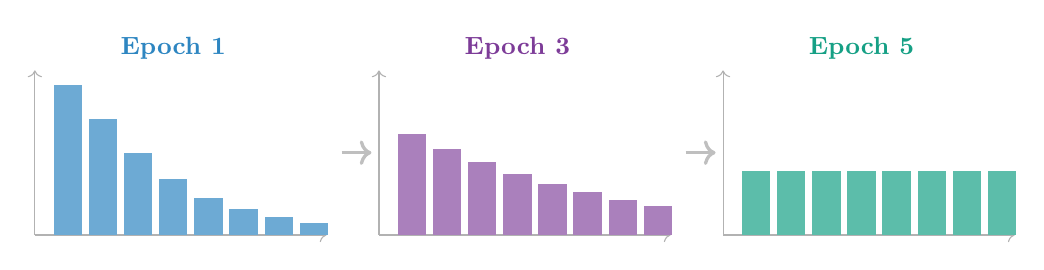
\begin{tikzpicture}[scale=0.95, every node/.style={font=\scriptsize}]
  \foreach \dx/\lbl/\col in {0/{Epoch 1}/contextblue, 4.6/{Epoch 3}/objectivepurple,
                             9.2/{Epoch 5}/methodteal} {
    \node[font=\small\bfseries,\col] at (\dx+1.85,2.5) {\lbl};
    \draw[->,gray!60] (\dx,0) -- (\dx+3.9,0);
    \draw[->,gray!60] (\dx,0) -- (\dx,2.2);
  }
  \foreach \x/\h in {0.25/2.0, 0.72/1.55, 1.19/1.1, 1.66/0.75, 2.13/0.5,
                     2.6/0.35, 3.07/0.24, 3.54/0.16}
    \fill[contextblue!70] (\x,0) rectangle (\x+0.38,\h);
  \foreach \x/\h in {4.85/1.35, 5.32/1.15, 5.79/0.98, 6.26/0.82, 6.73/0.68,
                     7.2/0.57, 7.67/0.47, 8.14/0.39}
    \fill[objectivepurple!65] (\x,0) rectangle (\x+0.38,\h);
  \foreach \x in {9.45,9.92,10.39,10.86,11.33,11.8,12.27,12.74}
    \fill[methodteal!70] (\x,0) rectangle (\x+0.38,0.85);
  \draw[->,very thick,gray!50] (4.1,1.1) -- (4.5,1.1);
  \draw[->,very thick,gray!50] (8.7,1.1) -- (9.1,1.1);
\end{tikzpicture}
\vspace{6pt}

\begin{columns}[T]
\begin{column}{0.46\textwidth}
  \begin{objectiveblock}{Tỉ lệ che tăng dần}
    \[ \mathcal{R}_m = e \times \mathcal{R}_s \]
    {\scriptsize $e$ là số epoch. Càng về sau che càng nhiều head.}
  \end{objectiveblock}
\end{column}
\begin{column}{0.5\textwidth}
  \begin{methodblock}{Mục tiêu}
    Phân phối nhãn \emph{còn lại} dịch dần từ \emphkey{đuôi dài} sang
    \emphok{đều}.
  \end{methodblock}
\end{column}
\end{columns}
\vspace{4pt}
\muted{\scriptsize Đây là \emph{Curriculum-Guided Mask Generation} --- đóng góp
thứ tư của bài. Nhớ slide này, lát nữa quay lại.}
\end{frame}

\begin{frame}{Một bộ ba chạy qua mô hình}
\centering
\begin{tikzpicture}[scale=0.95, every node/.style={font=\scriptsize},
   bx/.style={rounded corners=3pt, draw, minimum height=0.95cm,
              text width=2.15cm, align=center, inner sep=3pt}]
  \node[bx, draw=gray!60, fill=gray!8]              (a) at (0,0)   {khung $I^{12}$\\{\tiny người, cốc}};
  \node[bx, draw=contextblue, fill=contextblue!10]  (b) at (2.9,0) {ORPU + STPU\\{\tiny $\mathbf{z}_{ij}^{12}$}};
  \node[bx, draw=methodteal, fill=methodteal!12]    (c) at (5.8,0) {Decoder\\{\tiny $\hat{\mathbf{p}}_{ij}^{12}$}};
  \node[bx, draw=riskred, fill=riskred!10, text width=2.5cm] (d) at (9.0,0)
       {\textbf{Masked Loss}};
  \foreach \x/\y in {a/b, b/c, c/d} \draw[->,thick,gray!65] (\x) -- (\y);
  \draw[decorate,decoration={brace,amplitude=4pt},contextblue]
        (1.6,0.7) -- (6.9,0.7)
        node[midway,above=4pt,contextblue,font=\scriptsize\bfseries]
        {lấy nguyên từ mô hình nền --- forward pass KHÔNG đổi};

  \node[align=left, font=\scriptsize, text width=4.6cm] at (9.0,-1.9)
       {nhãn thật \textsf{looking\_at} $\to$ \textbf{head}\\
        $\Rightarrow \mathbf{m}=1 \Rightarrow \widetilde{\mathcal{L}}=0$};
  \draw[->,thick,riskred] (9.0,-1.35) -- (9.0,-0.5);
\end{tikzpicture}
\vspace{16pt}

\begin{methodblock}{Vì sao gắn được lên mọi mô hình}
  ImparTail \emphok{chỉ đổi backward}. Bài báo chứng minh bằng cách gắn lên
  \textbf{sáu} mô hình nền: STTran \cit{5}, DSGDetr \cit{6}, SceneSayer ODE/SDE \cit{4}\ldots
\end{methodblock}
\end{frame}

\begin{frame}{Kết quả --- cải thiện ở mọi ô}
\centering
{\small
\begin{tabular}{@{}l l ccc c ccc@{}}
  \toprule
  & & \multicolumn{3}{c}{\textbf{With Constraint}} & &
      \multicolumn{3}{c}{\textbf{No Constraint}} \\
  \cmidrule(lr){3-5}\cmidrule(lr){7-9}
  Mode & Method & mR@10 & mR@20 & mR@50 & & mR@10 & mR@20 & mR@50 \\
  \midrule
  \multirow{2}{*}{SGDET}
    & STTran       & 8.0 & 16.6 & 19.3 & & 19.3 & 26.9 & 35.6 \\
  \rowcolor{GoodBg}
    & \;+ImparTail & \textbf{9.4} & \textbf{21.5} & \textbf{25.9} & &
                     \textbf{23.5} & \textbf{33.6} & \textbf{43.8} \\
  \midrule
  \multirow{2}{*}{SGCLS}
    & STTran       & 25.0 & 27.5 & 27.6 & & 38.8 & 47.1 & 59.9 \\
  \rowcolor{GoodBg}
    & \;+ImparTail & \textbf{32.3} & \textbf{36.2} & \textbf{36.2} & &
                     \textbf{47.4} & \textbf{62.2} & \textbf{66.6} \\
  \midrule
  \multirow{2}{*}{PREDCLS}
    & STTran       & 30.5 & 34.7 & 34.7 & & 48.5 & 63.4 & 80.5 \\
  \rowcolor{GoodBg}
    & \;+ImparTail & \textbf{44.0} & \textbf{52.7} & \textbf{52.9} & &
                     \textbf{65.5} & \textbf{82.0} & \textbf{93.0} \\
  \bottomrule
\end{tabular}}
\vspace{8pt}

\begin{columns}[T]
\begin{column}{0.5\textwidth}
  \begin{methodblock}{mR@10 tăng}
    SGDET \textbf{12\%} $\cdot$ SGCLS \textbf{22\%} $\cdot$ PREDCLS \textbf{20\%}
  \end{methodblock}
\end{column}
\begin{column}{0.46\textwidth}
  \muted{\scriptsize SGA cũng tăng 12--20\%. Bảng đầy đủ ở \cit{1}.}
\end{column}
\end{columns}
\end{frame}

\begin{frame}{Độ bền --- tác vụ đánh giá mới bài báo đặt ra}
\begin{columns}[T]
\begin{column}{0.44\textwidth}
  \begin{objectiveblock}{Robust VidSGG / SGA}
    Huấn luyện trên dữ liệu \emph{sạch}, đánh giá trên khung hình
    \emphobj{đã làm nhiễu}.
  \end{objectiveblock}
  \vspace{4pt}
  {\scriptsize 16 kiểu nhiễu: cảm biến, thời tiết, ánh sáng.}
  \vspace{5pt}
  \begin{methodblock}{Kết quả}
    Điểm \emphok{sau khi nhiễu} của ImparTail vẫn cao hơn điểm \emph{sạch} của
    mô hình nền.
  \end{methodblock}
\end{column}
\begin{column}{0.53\textwidth}
  \centering
  \begin{tikzpicture}[scale=1.0, every node/.style={font=\scriptsize}]
    \draw[->,gray] (0,0) -- (0,3.5) node[above,font=\scriptsize]{mR@10};
    \draw[->,gray] (0,0) -- (5.2,0);
    \node at (1.3,-0.35) {sạch}; \node at (3.7,-0.35) {nhiễu Gaussian};
    \fill[gray!55]       (0.6,0) rectangle (1.3,2.29);
    \fill[gray!55]       (3.0,0) rectangle (3.7,1.57);
    \draw[gray,dashed,thick]  (1.3,2.29) -- (3.0,1.57);
    \node[gray,font=\scriptsize\bfseries] at (2.15,2.25) {STTran $-14.3$};
    \fill[methodteal!75] (1.4,0) rectangle (2.1,3.28);
    \fill[methodteal!75] (3.8,0) rectangle (4.5,2.88);
    \draw[methodteal,dashed,thick] (2.1,3.28) -- (3.8,2.88);
    \node[methodteal,font=\scriptsize\bfseries] at (2.95,3.5) {+ImparTail $-8.0$};
    \node[font=\tiny,gray]       at (0.95,-0.72) {45.7};
    \node[font=\tiny,gray]       at (3.35,-0.72) {31.4};
    \node[font=\tiny,methodteal] at (1.75,-0.72) {65.5};
    \node[font=\tiny,methodteal] at (4.15,-0.72) {57.5};
  \end{tikzpicture}
\end{column}
\end{columns}
\end{frame}

\begin{frame}{Đọc phản biện --- curriculum có được dùng không?}
\begin{alertblock}{Remark, trang 7 của bài báo \cit{1}}
  {\itshape ``\ldots a fixed Stochastic Masking Ratio of 0.9 achieved
  \textbf{similar performance} \ldots Therefore, in the paper to report results,
  we opted for a \textbf{fixed Masking Ratio of 0.9}.''}
\end{alertblock}
\vspace{6pt}

\centering
\begin{tikzpicture}[scale=0.95, every node/.style={font=\scriptsize},
   ev/.style={rounded corners=3pt, draw=riskred!70, fill=riskred!8,
              text width=3.3cm, align=center, minimum height=1.1cm, inner sep=4pt}]
  \node[ev] (a) at (0,0)   {\textbf{Bài báo}\\Remark trang 7};
  \node[ev] (b) at (4.0,0) {\textbf{Mã nguồn}\\\texttt{is\_curriculum = False}};
  \node[ev] (c) at (8.0,0) {\textbf{Script chạy}\\không gọi curriculum};
  \node[riskred,font=\small\bfseries] at (4.0,-1.25) {ba nguồn độc lập, cùng kết luận};
\end{tikzpicture}
\vspace{16pt}

\begin{riskblock}{Câu hỏi để lại}
  Curriculum là \emphwarn{đóng góp thứ tư} và chiếm một phần tư Hình 3 --- nhưng
  số trong bảng chính đến từ tỉ lệ cố định. Vậy đóng góp thật nằm ở
  \emph{curriculum} hay chỉ ở \emph{việc che}?
\end{riskblock}
\vspace{2pt}
\muted{\tiny Đây là mô tả bài báo và mã đã công bố, không kết luận về việc tác
giả đã chạy gì trong nghiên cứu.}
\end{frame}

\begin{frame}{Nhóm chạy lại được --- 9 con số khớp Bảng 1}
\centering
\begin{tabular}{lccc}
\toprule
\textbf{ràng buộc} & \textbf{mR@10} & \textbf{mR@20} & \textbf{mR@50}\\
\midrule
With & 30,5 $\to$ \textbf{30,7} & 34,7 $\to$ \textbf{35,5} & 34,8 $\to$ \textbf{35,6}\\
No   & 45,7 $\to$ \textbf{44,3} & 63,4 $\to$ \textbf{63,8} & 80,5 $\to$ \textbf{80,7}\\
Semi & 36,6 $\to$ \textbf{36,2} & 51,8 $\to$ \textbf{52,7} & 53,8 $\to$ \textbf{55,3}\\
\bottomrule
\end{tabular}
\vspace{10pt}

\begin{block}{Điều kiện}
Toàn bộ \textbf{1.750 video} tập test $\cdot$ chế độ PredCls $\cdot$ checkpoint
do tác giả phát hành $\cdot$ khoảng một giờ trên Tesla P100.
\end{block}
\vspace{4pt}

Lệch trung bình \textbf{0,74 điểm}, lớn nhất 1,52.
Đây là mô hình \emph{nền} STTran --- nhóm chưa chạy bản có phương pháp.
\vspace{6pt}

\muted{\tiny Ba rào cản tưởng chặn đường hoá ra không phải: dữ liệu có sẵn trên
Kaggle, checkpoint tải được, CUDA extension biên dịch sạch sau khi vá 51 chỗ
dùng API đã bỏ.}
\end{frame}

\begin{frame}{Ba điều mang về}
\vspace{6pt}
\begin{objectiveblock}{Đổi mục tiêu, đừng đổi kiến trúc}
  Một phép nhân với mặt nạ nhị phân. \emphobj{Không thêm tham số nào},
  mean Recall tăng 12--22\%.
\end{objectiveblock}
\vspace{6pt}
\begin{methodblock}{Chỉ số quyết định điều mình nhìn thấy}
  Recall giấu điểm yếu ở đuôi. \emphok{mean Recall} phơi ra.
\end{methodblock}
\vspace{6pt}
\begin{riskblock}{Đọc bài báo cùng với mã}
  Phát hiện về curriculum \emphwarn{chỉ hiện ra khi đọc cả hai}.
\end{riskblock}
\end{frame}

\begin{frame}{Tài liệu tham khảo}
{\footnotesize
\begin{enumerate}\itemsep4pt
  \item R. Peddi, Saurabh, A. A. Shrivastava, P. Singla, and V. Gogate,
        ``Towards unbiased and robust spatio-temporal scene graph generation and
        anticipation,'' in \emph{Proc. IEEE/CVF Conf. Comput. Vis. Pattern
        Recognit. (CVPR)}, 2025.
  \item J. Ji, R. Krishna, L. Fei-Fei, and J. C. Niebles, ``Action Genome:
        Actions as compositions of spatio-temporal scene graphs,'' in
        \emph{Proc. IEEE/CVF Conf. Comput. Vis. Pattern Recognit. (CVPR)}, 2020.
  \item G. A. Sigurdsson, G. Varol, X. Wang, A. Farhadi, I. Laptev, and A.
        Gupta, ``Hollywood in homes: Crowdsourcing data collection for activity
        understanding,'' in \emph{Proc. Eur. Conf. Comput. Vis. (ECCV)}, 2016.
  \item R. Peddi, S. Saurabh, P. Singla, and V. Gogate, ``Towards scene graph
        anticipation,'' in \emph{Proc. Eur. Conf. Comput. Vis. (ECCV)}, 2024.
  \item Y. Cong, W. Liao, H. Ackermann, B. Rosenhahn, and M. Y. Yang,
        ``Spatial-temporal transformer for dynamic scene graph generation,'' in
        \emph{Proc. IEEE/CVF Int. Conf. Comput. Vis. (ICCV)}, 2021.
  \item S. Feng, H. Mostafa, M. Nassar, S. Majumdar, and S. Tripathi,
        ``Exploiting long-term dependencies for generating dynamic scene
        graphs,'' in \emph{Proc. IEEE/CVF Winter Conf. Appl. Comput. Vis.
        (WACV)}, 2023.
\end{enumerate}}
\vspace{4pt}
\muted{\scriptsize Toàn bộ hình trong bộ slide này do nhóm tự vẽ bằng TikZ, không
dùng ảnh từ nguồn ngoài hay ảnh tạo sinh bởi AI. Số liệu trong bảng lấy từ Bảng 1
và Bảng 3 của \cit{1}.}
\end{frame}

\end{document}
